\documentclass[tikz, border=2pt]{standalone}
\begin{document}
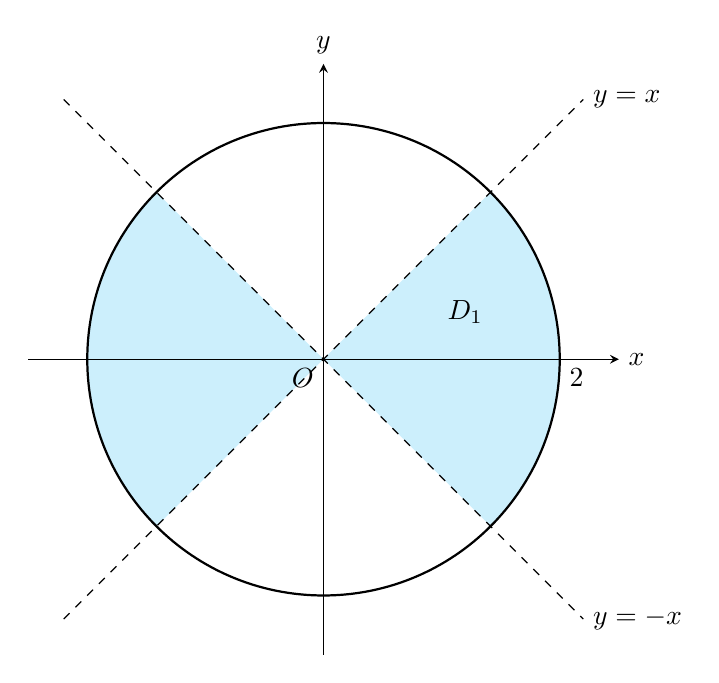
\begin{tikzpicture}[scale=1.5, >=stealth]
    % 填充积分区域 D (左右两个扇形)
    \fill[cyan!20] (0,0) -- (45:2) arc (45:-45:2) -- cycle;
    \fill[cyan!20] (0,0) -- (135:2) arc (135:225:2) -- cycle;

    % 画坐标轴
    \draw[->] (-2.5,0) -- (2.5,0) node[right] {$x$};
    \draw[->] (0,-2.5) -- (0,2.5) node[above] {$y$};

    % 画单位圆边界
    \draw[thick] (0,0) circle (2);
    
    % 画分界线 |x| = |y| 即 y = x 和 y = -x
    \draw[dashed] (-2.2,-2.2) -- (2.2,2.2) node[right] {$y=x$};
    \draw[dashed] (-2.2,2.2) -- (2.2,-2.2) node[right] {$y=-x$};

    % 标注
    \node at (1.2,0.4) {$D_1$};
    \node[below left] at (0,0) {$O$};
    \node[below right] at (2,0) {$2$};
\end{tikzpicture}
\end{document}